% Created 2021-09-27 Mon 12:03
% Intended LaTeX compiler: xelatex
\documentclass[letterpaper]{article}
\usepackage{graphicx}
\usepackage{grffile}
\usepackage{longtable}
\usepackage{wrapfig}
\usepackage{rotating}
\usepackage[normalem]{ulem}
\usepackage{amsmath}
\usepackage{textcomp}
\usepackage{amssymb}
\usepackage{capt-of}
\usepackage{hyperref}
\setlength{\parindent}{0pt}
\usepackage[margin=1in]{geometry}
\usepackage{fontspec}
\usepackage{svg}
\usepackage{cancel}
\usepackage{indentfirst}
\setmainfont[ItalicFont = LiberationSans-Italic, BoldFont = LiberationSans-Bold, BoldItalicFont = LiberationSans-BoldItalic]{LiberationSans}
\newfontfamily\NHLight[ItalicFont = LiberationSansNarrow-Italic, BoldFont       = LiberationSansNarrow-Bold, BoldItalicFont = LiberationSansNarrow-BoldItalic]{LiberationSansNarrow}
\newcommand\textrmlf[1]{{\NHLight#1}}
\newcommand\textitlf[1]{{\NHLight\itshape#1}}
\let\textbflf\textrm
\newcommand\textulf[1]{{\NHLight\bfseries#1}}
\newcommand\textuitlf[1]{{\NHLight\bfseries\itshape#1}}
\usepackage{fancyhdr}
\pagestyle{fancy}
\usepackage{titlesec}
\usepackage{titling}
\makeatletter
\lhead{\textbf{\@title}}
\makeatother
\rhead{\textrmlf{Compiled} \today}
\lfoot{\theauthor\ \textbullet \ \textbf{2021-2022}}
\cfoot{}
\rfoot{\textrmlf{Page} \thepage}
\renewcommand{\tableofcontents}{}
\titleformat{\section} {\Large} {\textrmlf{\thesection} {|}} {0.3em} {\textbf}
\titleformat{\subsection} {\large} {\textrmlf{\thesubsection} {|}} {0.2em} {\textbf}
\titleformat{\subsubsection} {\large} {\textrmlf{\thesubsubsection} {|}} {0.1em} {\textbf}
\setlength{\parskip}{0.45em}
\renewcommand\maketitle{}
\author{Houjun Liu}
\date{\today}
\title{Limits}
\hypersetup{
 pdfauthor={Houjun Liu},
 pdftitle={Limits},
 pdfkeywords={},
 pdfsubject={},
 pdfcreator={Emacs 28.0.50 (Org mode 9.4.4)}, 
 pdflang={English}}
\begin{document}

\tableofcontents



\section{Limits}
\label{sec:org6e912e6}
\subsection{Warming up}
\label{sec:org5dcc6af}
Here's a function

\(y = \frac{1}{x}\).

We know that it has

\begin{itemize}
\item Domain \(D (-\infty, 0)(0, \infty)\)
\item Range \(R (-\infty, 0)(0, \infty)\)
\item \(As\ x\to\infty,\ y\to0\)
\item Function is \emph{odd}, that is, \(f(-x) = -f(x)\)
\end{itemize}

\subsection{The Limit Notation}
\label{sec:org82174fb}
See \href{KBhMATH401TheLimitNotation.org}{KBhMATH401TheLimitNotation}

\subsection{Computing Limits Algebraically}
\label{sec:orgfebe03c}
See \href{KBMATH401ComputingLimits.org}{KBMATH401ComputingLimits}

\subsection{Types of Discontinuity}
\label{sec:org3907fe2}
See \href{KBhMATH401Discontinuity.org}{KBhMATH401Discontinuity}

\subsection{Error and Epsilon Delta Proofs}
\label{sec:org15e5810}
See
\href{KbhMATH401EpsilonDeltaProofs.org}{KbhMATH401EpsilonDeltaProofs}

\subsection{CN10062020 Continuity}
\label{sec:orgedd8739}
\#disorganized \#flo

\(\lim_{x \to a} f(x) \neq f(a)\).

Sometimes

*A function is continuous at \(x=a\) if ALL OF the following three
conditions:\$

\begin{enumerate}
\item \(\lim_{x\to a} f(x)\) exists
\item \(f(a)\) exists
\item \(\lim_{x\to a} f(x) = f(a)\)
\end{enumerate}

\begin{figure}[htbp]
\centering
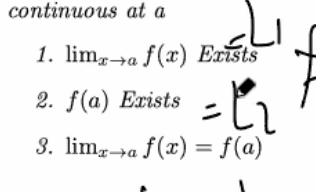
\includegraphics[width=.9\linewidth]{threestepslimit.png}
\caption{threestepslimit.png}
\end{figure}

\definition{Removable discontinuity}{Removeable discontinuity are often holes. They are discontinuities that, with an additional definition, one could remove.}
For instance, \(f(x) = \frac{x^2-x-2}{x-2}\) has a hole at \(x=2\), but
if we defined a value for \(x=2\), our lovely discontinuity is
immediately removed.

\defintion{Infitinite discontinuity}{Functions that approch infinity}
If you think about it, if you try to fix the discontinuity, you will be
tracing all the way up the infinity

\definition{Jump discontinuity}{"Staircase" functions that causes jump}
Like\ldots{}

\begin{figure}[htbp]
\centering
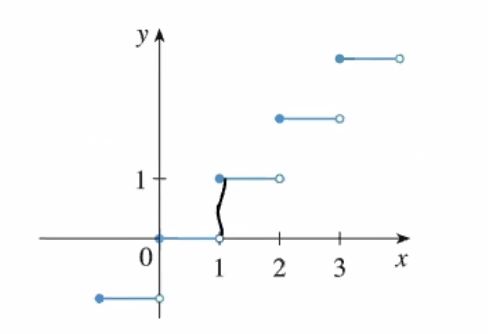
\includegraphics[width=.9\linewidth]{jumpdisc.png}
\caption{jumpdisc.png}
\end{figure}

As you could see, if you try to fix the discontinuity, this would result
in vertical lines, which is illegal in functions.

\textbf{Continuous-from-right}: \(f(a) = \lim{x \to a^+} f(x)\)
\textbf{Continuous-from-left}: \(f(a) = \lim{x \to a^-} f(x)\)
\end{document}
